\documentclass[problem]{mcs}

\begin{pcomments}
    \pcomment{TP_Random_Walks}
    \pcomment{Converted from random-walks.scm
              by scmtotex and dmj
              on Sun 13 Jun 2010 05:25:50 PM EDT}
    \pcomment{fig: relabeled ARM 8/24/11}
    \pcomment{subsumed by CP_random_walk_stationary_distributions_F13}
\end{pcomments}

\begin{problem}
Consider the following random-walk graphs:
\begin{center}
\begin{figure}[h!]
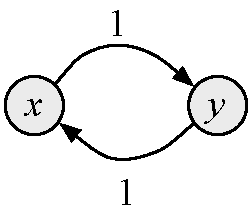
\includegraphics[height=20mm]{randomWalkFigs/bipart.pdf}
\caption{\label{fig:Ran_bipart}}
\end{figure}
\begin{figure}[h!]
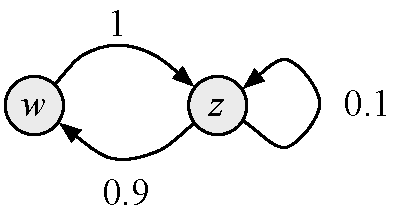
\includegraphics[height=20mm]{randomWalkFigs/stable.pdf}
\caption{\label{fig:Ran_stable}}
\end{figure}
\begin{figure}[h!]
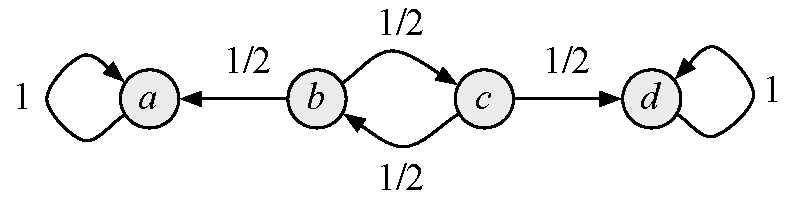
\includegraphics[height=20mm]{randomWalkFigs/sinky.pdf}
\caption{\label{fig:Ran_sinky}}
\end{figure}
\end{center}

\bparts

\ppart
Find $d(x)$ for a stationary distribution for graph \ref{fig:Ran_bipart}.

\begin{solution}
1/2
\end{solution}

\ppart
Find $d(y)$ for a stationary distribution for graph \ref{fig:Ran_bipart}.

\begin{solution}
1/2
\end{solution}

\ppart

If you start at node $x$ in graph \ref{fig:Ran_bipart} and take a (long) random walk,
does the distribution over nodes ever get close to the stationary
distribution?

\begin{solution}
No, you will just alternate between nodes $x$ and $y$.
\end{solution}

\ppart
Find $d(w)$ for a stationary distribution for graph \ref{fig:Ran_stable}.

\begin{solution}
9/19

Found by solving $d(w)=.9d(z)$, $d(z)=d(w)+.1d(z)$ and $d(w)+d(z)=1$
simultaneously.
\end{solution}

\ppart

Find $d(z)$ for a stationary distribution for graph \ref{fig:Ran_stable}.

\begin{solution}
10/19
\end{solution}

\ppart

If you start at node $w$ in graph \ref{fig:Ran_stable} and take a (long) random walk,
does the distribution over nodes ever get close to the stationary
distribution?  (\hint try a few steps and watch what is happening.)

\begin{solution}
Yes
\end{solution}

\ppart

How many stationary distributions are there for graph
\ref{fig:Ran_sinky}?

\begin{solution}
infinitely many
\end{solution}

\ppart

If you start at node $b$ in graph \ref{fig:Ran_sinky} and take a
(long) random walk, what will be the approximate probability that you
are at node $d$?

\begin{solution}
1/3
\end{solution}

\eparts

\end{problem}

\endinput
